\documentclass[12pt]{report}
\usepackage{geometry}
\usepackage{graphicx,amsmath,amssymb,amsfonts,listings,color}
\usepackage{graphics}
\usepackage{xcolor}
\usepackage[screen,nopanel]{pdfscreen}
\usepackage[normalem]{ulem}
\usepackage{listings}
\usepackage{titlesec}
\usepackage{hyperref}
\titleformat{\section}
{\color{blue}\normalfont\Large\bfseries}
{\color{blue}\thesection}{1em}{}

\geometry{left=15mm,right=15mm}


 
\title{\textbf{Indian Institute of Information Technology,Vadodara\\} \color{blue}Science and Morality in shelley's frankenstein: Consequences of Technology} 

\date{\today}
\author{By-\\ Govind Kumar Meena\\B.Tech-IT(3rd year)} 

\begin{document}
\maketitle

\tableofcontents
\newpage
\section{Acknowledgement:}
\LARGE
I would like to take this opportunity to express my very deep gratitude and deep regard to my guide or instructor Dr.Barnali chetia, for her very good guidance, valuable feedback and constant encouragement throughout the duration of the project. Her valuable suggestions were of extremely great help throughout my project work. Her perceptive criticism kept me working to make this project in a much better way. Working under her was an extremely knowledgeable experience for me.\\
I would also like to give my sincere gratitude to IIIT-Vadodara and all the friends and colleagues who filled in the survey, without which this research would be incomplete.

\newpage
\section{Abstract:}
\LARGE
This research paper will show you that how people thinks about science and morality. You will know that  people are often wrong about science (i.e. rejecting evolution) people are often wrong about what is moral.
This paper will help you to understand moral judgement that people oftenaly thinks science does not make any judgement.
It will help you understanding about consequences of scientific research.
We all know that consequences can be right and wrong but results always comes either it's right or wrong.  

\newpage
\section{Introduction:}
\LARGE
                    Science always used for some bad purposes as good ones.we must never forget that humankind not only defined by intelligence only also by a person's moral sense of right and wrong. we know that powers of science are morally natural and widely held and advanced by scientists.They leave it up to others to decide how to use them. "Science can only make sure of what is, but not what should be," Albert Einstein said, "and outside of its domain value judgments of all kinds remain necessary."
\\

However people are often struggle to determine what is right and what is wrong ?
\\

Decision that involve tension between moral principles can generates cognitive conflict within a person and ignite disagreement between peoples moral belief in given situation.
\\
In the starting of the story mary shelley describes that frankenstein thought about some innovations using parts of deadbodies or we can say making a human from the death and give him powers that can only given by God only. So for that he learned all of the science behind the human life. And he believes that with these scientific powers human kind would have some advantages or would be served with the positive effects.
So there is a situation in mary shelley's frankenstein where Victor frankenstein was not able to take decision that's why he is building that human life. He was only thinking of building a human that can help people and he will be the God for him but never thought of wrong aspects like "what if he will be harmfull to the humankind ?". 
\\

So what had heppened in the frankenstein we have learned that we can't take on the role of God. Victor frankenstein tried to create a life from death and the consequences were dreadfull.  He tried to go against the natural order. Sometimes scientific research and success has serious implications like atomic bombs.\\

When monster ask Victor frankenstein to create a companion for him though, Victor feels it's not morally right, even though that would save his family and himself.

\section{Overview:}

\subsection{Morality and science in mary shelley's frankenstein:}
                                                             “The Frankenstein” written by mary shelley is the book of single minded thoughts,the whole novel is about the very state of the mind of frankenstein.The whole story of  this book is stands on a perticular minds only one thought is "how life comes in a human body."
\\

The main character of the book is Victor Frankenstein and he has only one thing in his mind is about the  scientific technological knowledge. His mind was filled with only one perticuler thought of investing new scientific achievements. And he spends his most of the time with working on his target.He had only one think in his mind is that i want to create a human life using technology and science he learned or knowledge he has. He never thought of morality and what can be the consequences of his work that will be done by him later.He created a monster using that knowledge of science and technology he has, and he leaved  him behind in the laboratory.The monster had already ran away and made damages on the local townsman and killed most of Doctor Frankenstein’s family and friends.
\\

Morallity had always been questioned by people.Yet till this day not one of us can say what is morally right? 
\\

In the book "the frankenstein" by mary shelley Frankenstein knows that it was morally right to not create another monster.Doctor does not begin his work on second monster because he had a fear of killing his family by first monster. The monster angrily said to Frankenstein, “I can make you so wretched” (Shelley 162). The monster killed one of his friend cherval because monster knows that he was so close to him and good friend and now he has fear of killing Elizabeth by monster while she was trying to sleep.\\

Frankenstein knew without a doubt that creating another monster would not be right. After Frankenstein saw the destruction that one monster made, he probably got a view of what two monsters could end up doing and that probably also made him chose to not to create the monster. With two monsters on the loose they could end up breeding and starting a new race of super evil soldiers that could end up wiping out Europe. The monsters can potentially take over whatever they please, "A race of devils be propagated."(163) 
\newpage
\section{Hypothesis:}
\LARGE
Science deals with empirical reality with what heppens in the world.
Science always predicts that it will be good for the people but its not always true sometimes it goes wrong it affects human bieng.
Every research leads to some positive and some negative consequences so science does make moral judgements but only for positive aspects like victor frankenstein never thought of  "what if it will be wrong for humankind ?".
\newpage
\section{Survey-}
\subsection{Sample size-}
\LARGE
40 participants of my college IIIT-V including students of  Ist year, IInd year, IIIrd year and some faculty also.\\

Age group of students are : 19-24 years\\

Age group of faculties are : 30-40 years \\ 

Female participants are 30\% \\

Male participants are 70\%
\\

\subsection{Method-}
\LARGE
Questionnaires
\newpage

\subsection{Survey Analysis-}
\LARGE
\subsubsection{}  According to survey report
50\% people thinks that science fiction is the human experience of science and its resultant technologies, 20\% thinks that Nightmares and visions,that makes you supernatural in your dreams is science fiction,10\% Science fiction is really sociological  studies of the future and rest 20\% thinks that anything above can be science fiction.\\
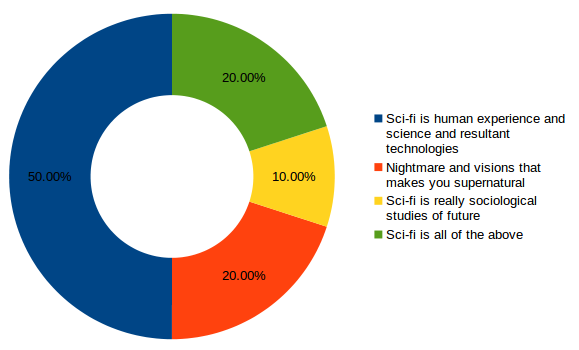
\includegraphics[width=5in,height=4in]{1.png}
\newpage
\LARGE

\subsubsection{} According to survey 74.5\% people thinks that science can answer moral questions and rest 24.5\% don't think that science can answer moral questions.
\\

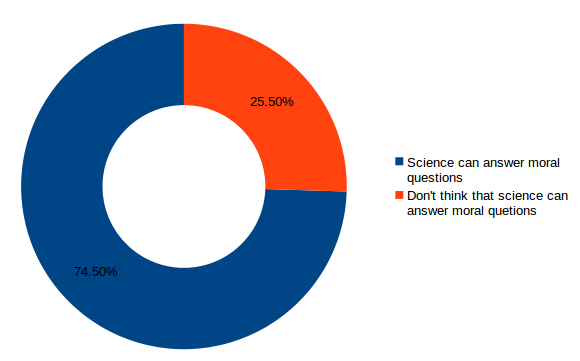
\includegraphics[width=5in,height=4in]{2.png}
\newpage
\LARGE

\subsubsection{} 50\% people believes that science believes in morality, 15\% people don't think that science believes in morality and rest 35\% said neither(sometimes it believes and sometimes doesn't).
\\

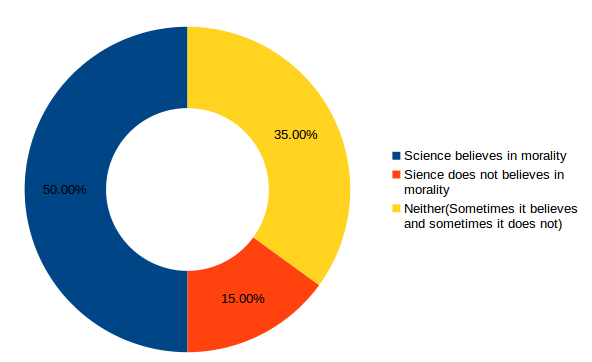
\includegraphics[width=5in,height=4in]{3.png}
\newpage
\LARGE

\subsubsection{} according to survey 35\% people said that science has limits, 35\% people said that it depends and 30\% people thinks not yet discovered.
\\
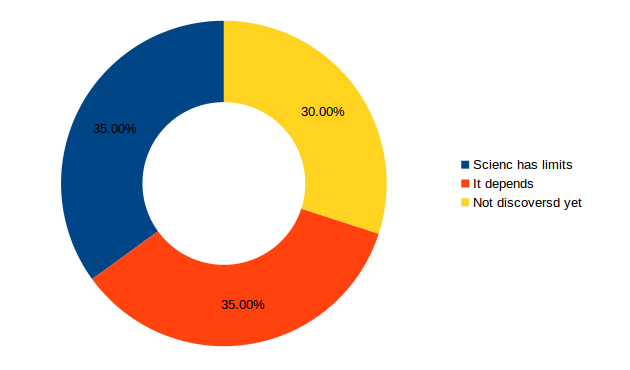
\includegraphics[width=5in,height=4in]{4.png}
\newpage
\LARGE

\subsubsection{}  60\% people thinks that science does not make moral judgement, instead of only 5\% people thinks it makes moral judgement and 35\% people said that sometime science make moral judgement and sometimes it's not.
\\

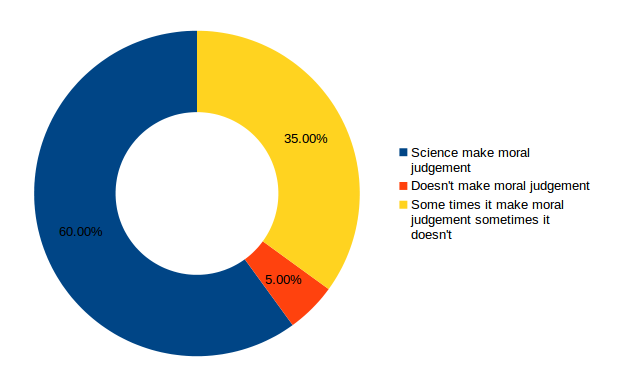
\includegraphics[width=5in,height=4in]{5.png}
\newpage
\LARGE

\subsubsection{}  90\% people believes that every scientific research have some consequences,5\% people said not every but some research have consequences and rest 5\% said that every scientific research always have object it can be good and bad.   
\\

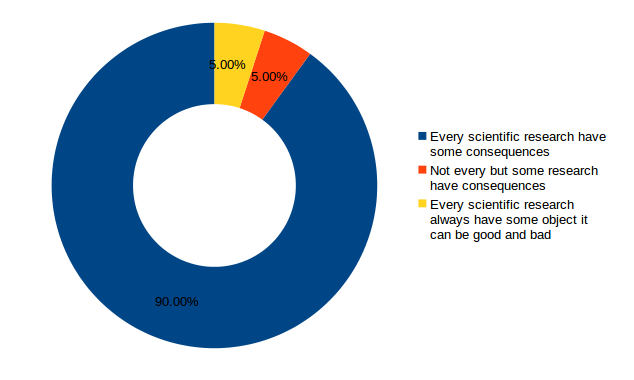
\includegraphics[width=5in,height=4in]{6.png}
\newpage
\LARGE

\subsection{Tools}
\LARGE
I have done this survey offline without using any tool and analyze it manually.

\subsection{Results}
\LARGE
As resultant people believes that science -fiction is a human experience of science and its resultant technologies and dreams that makes you supernatural.\\
Most people thinks that science has moral issues like sometimes thinks goes right and sometimes goes wrong.\\
Most people thinks that every scientifc research always have consequence it can be good or it can be bad.

\section{Litreture Review-}
\LARGE
Mary shelley wrote many novels including Lodore (1835), Faulkner (1937), Mathilde (1959), Valperga or the Life and Adventures of Castruccia, Prince of Lucca (1823), The Last Man (1826), and The Fortunes of Perkin Warbeck (1830). but none of her other works gained popularity as "Frankenstein" did. 
People also wrote some esseys and research papers on science and morality and about mary shelley's frankenstein, some of them are given here about what they did-
\\
\underline{Feminist Overtones in Mary Shelley's “Frankenstein”:}\\
\underline{The Symbolism in the Role of “Victor”} 
\\
	The author discussed of mary shelly's classic science fiction who contends that the underlying theme of crush could be interpreted to apply to the social situation which the feminist movement as a whole has revolted against. The primary perpetrator of this situation in Mary Shelly’s "Frankenstein" is identified as Dr. Victor Frankenstein, Frankenstein’s fictional creator.\\
	
\underline{The science in frankenstein-}
\\ 
In this paper auther films Frankenstein and The Bride of Frankenstein and contemplates the science as contained in each. Mary Shelley's original work is also discussed.\\

\underline{Shelly's Frankenstein/Dangers of Scientific Progress -}
\\
In this essay The writer argues Shelley's novel seems to speak directly to the modern reader and offer explicit warning against scientific discovery unregulated by restrictions of morality or responsibility. Victor Frankenstein, Shelley's brilliant scientist, suffers a tragic downfall worthy of the ancient Greek tragedians. Shelley's text suggests that this occurs due to two failings. First of all Frankenstein, like the ancient Greek tragic heroes, is guilty of hubris, that is, excessive pride, of "attempting to be like God" (Madigan 48), but also, he initially does not take responsibility for his actions. Furthermore, in his hubris, Frankenstein exhibits two characteristics that he himself castigates, "cowardice and carelessness," which he exhibits in the manner in which he deals with his creation (Shelley 37).\\

\underline{Science and Frankenstein:A faminist Prespctive-}
In this paper auther want to focus on Mary Shelly's famous work and the science that is portrayed in that book. Some of the science seen in the book has become more possible and more likely in recent years, whilst some is still fantasy. Perhaps one of the most interesting aspects of this papers examination of Frankenstein is the way that the science is presented when considered in the light of gender issues and the monster being seen as a possible feminist alter ego. \\

And Many more work has been done by peoples on mary shelley's frankenstein, science and morality.
\newpage
\section{Conclusion-}
Most of the time people thinks or believes that science believes in morality but not always some of inventions of science has disastorious effects on all over the world or on a part of society.
We know that for some experiments science has some limits but its not fully proved.
There are many evolution on human life but we can't guarantee on anyone.  
\newpage
\section{References-}
\begin{lstlisting}
http://www.directessays.com/viewpaper/9720.html?
ev=1&utm_expid=174881-6.F-Jepu57Ta-9ruf8-exf0Q.
1&utm_referrer=https%3A%2F%2Fwww.google.co.in

http://www.thenewatlantis.com/publications/
the-moral-challenge-of-modern-science
https://www.clas.ufl.edu/ipsa/2003/ginn.html
https://www.insidescience.org/content/
science-made-frankenstein/1116
https://en.wikipedia.org/wiki/Mary_Shelley
https://www.goodreads.com/work/quotes/
4836639-frankenstein-or-the-modern-prometheus
http://www.articlemyriad.com/analysis-frankenstein-mary-shelley/
http://www.autodidactproject.org/other/arsenyev1.html
http://carneades.pomona.edu/1998-2006/2006
Ethics/Notes/Harman.shtml
\end{lstlisting}
\section{Appendix-}
\subsection{Appendix-A}
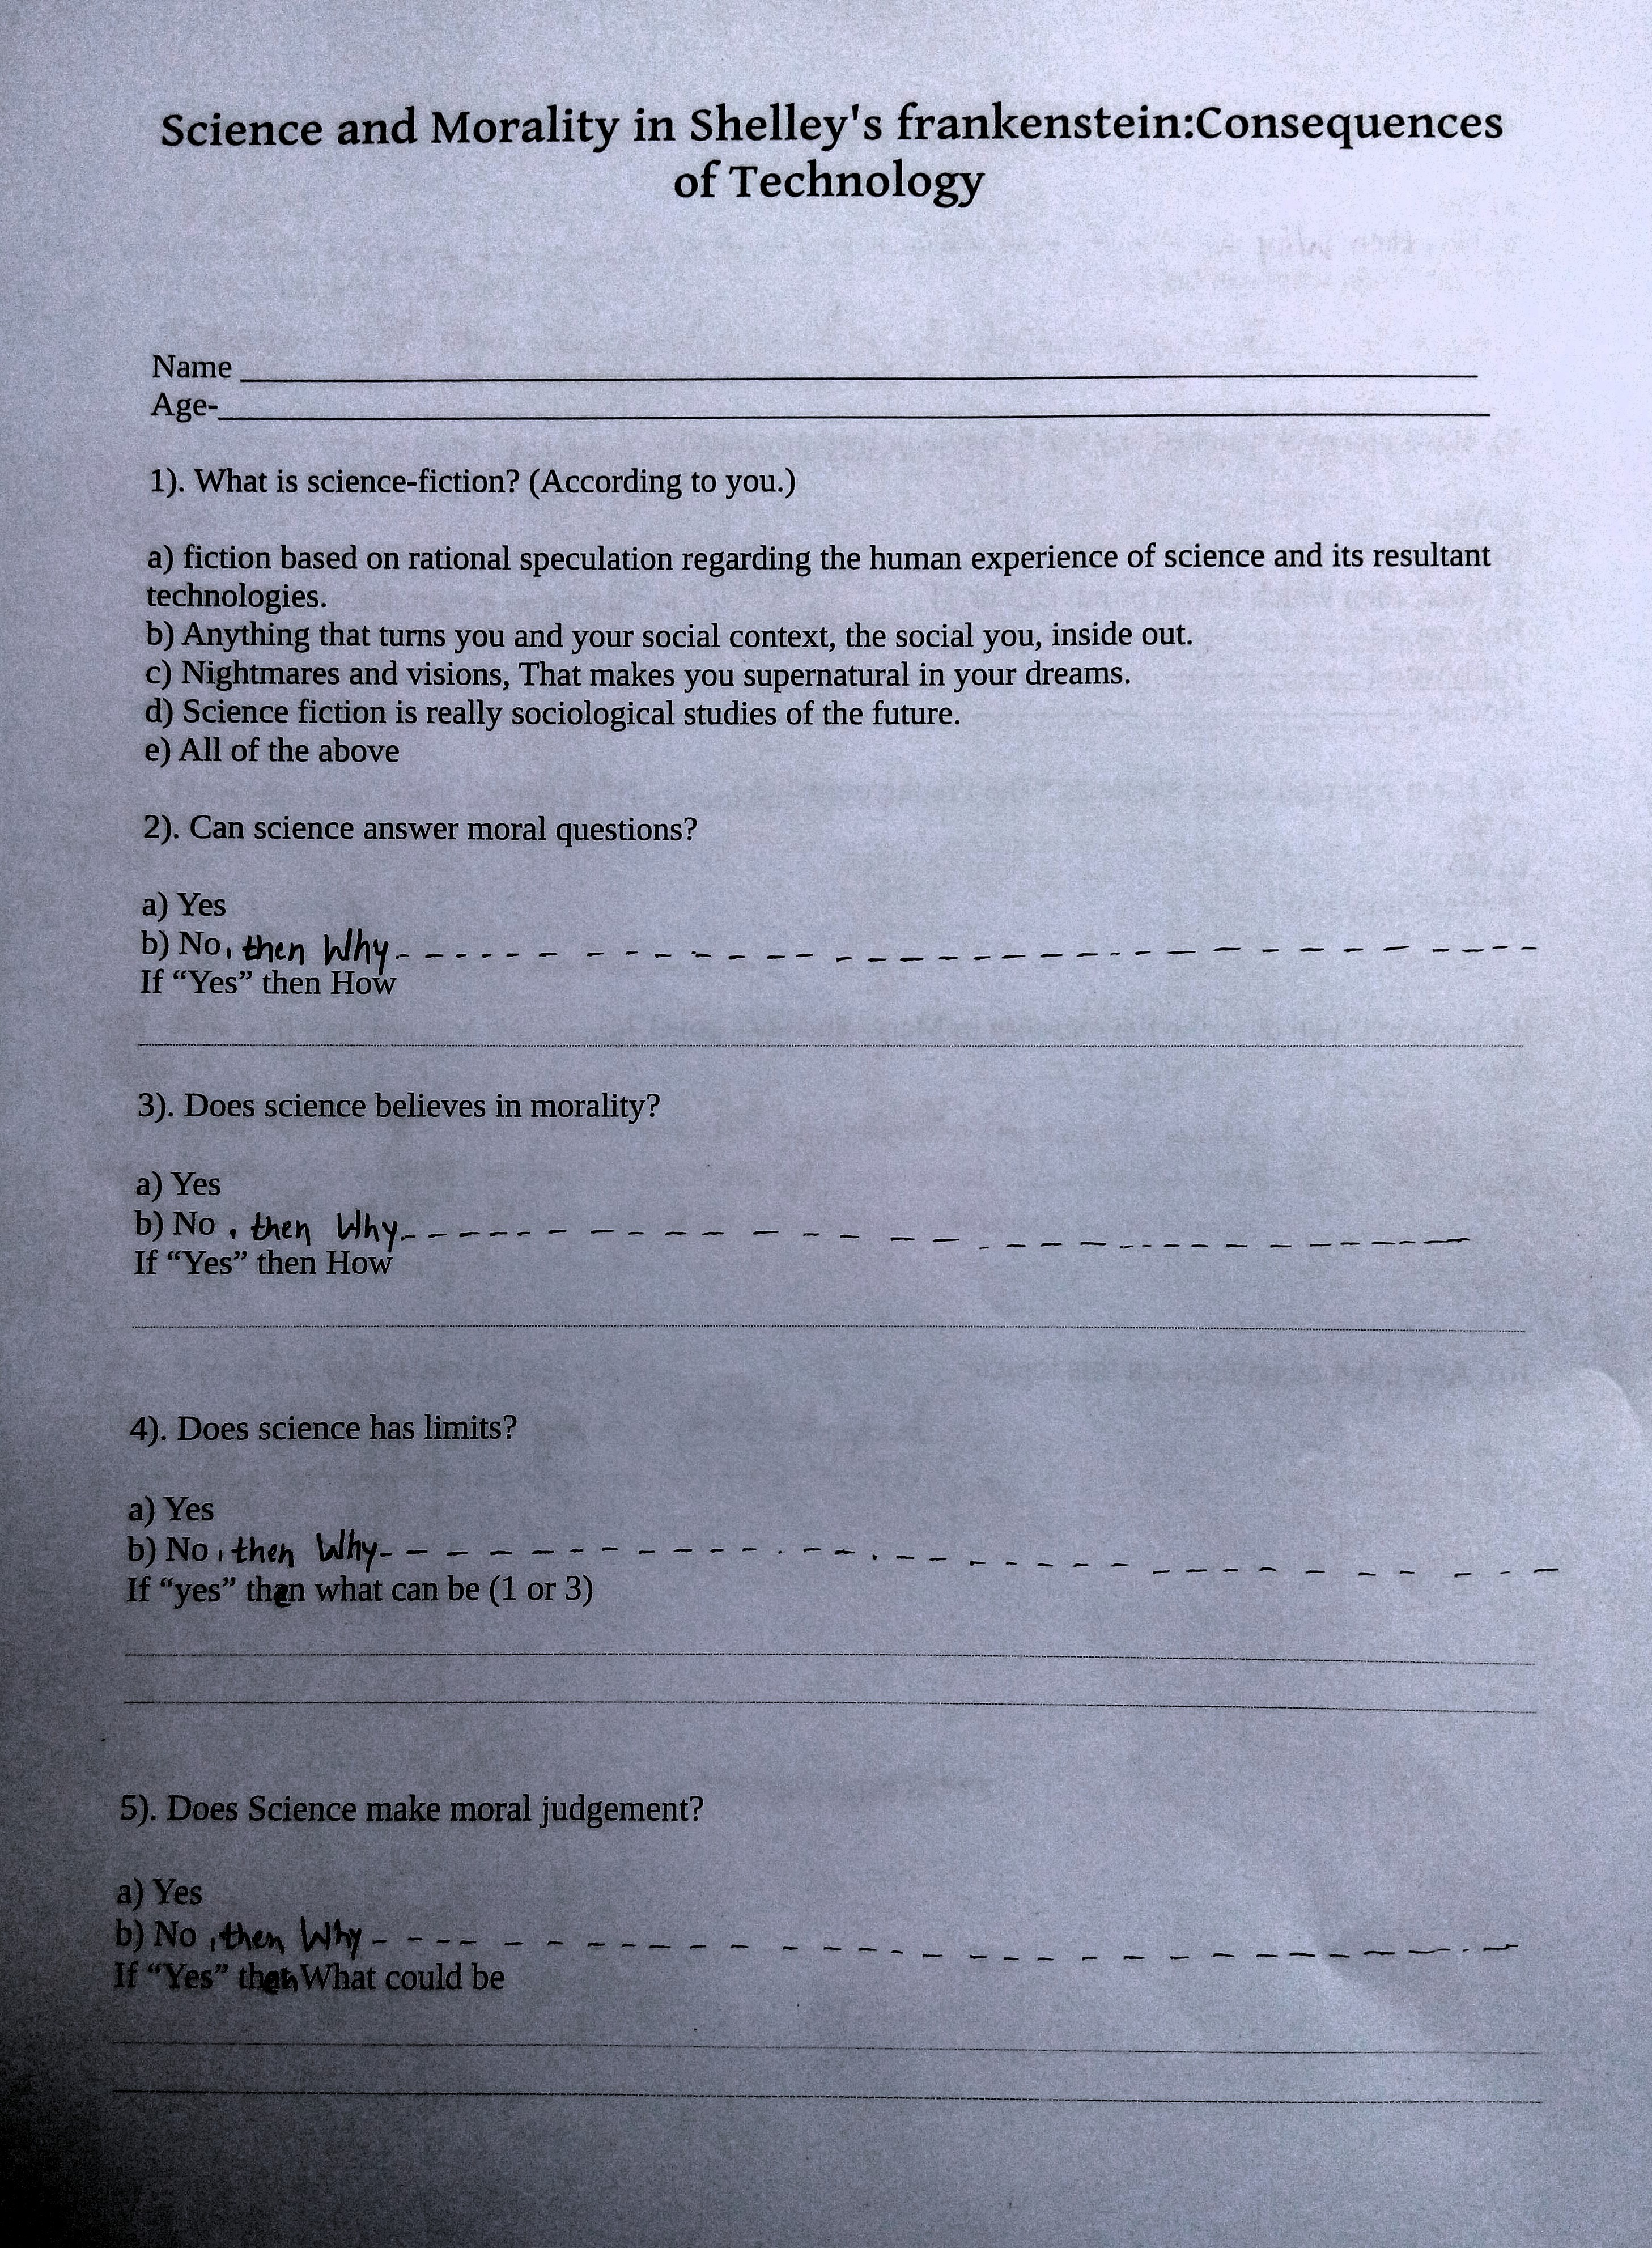
\includegraphics[width=6in,height=7in]{a1.jpg}

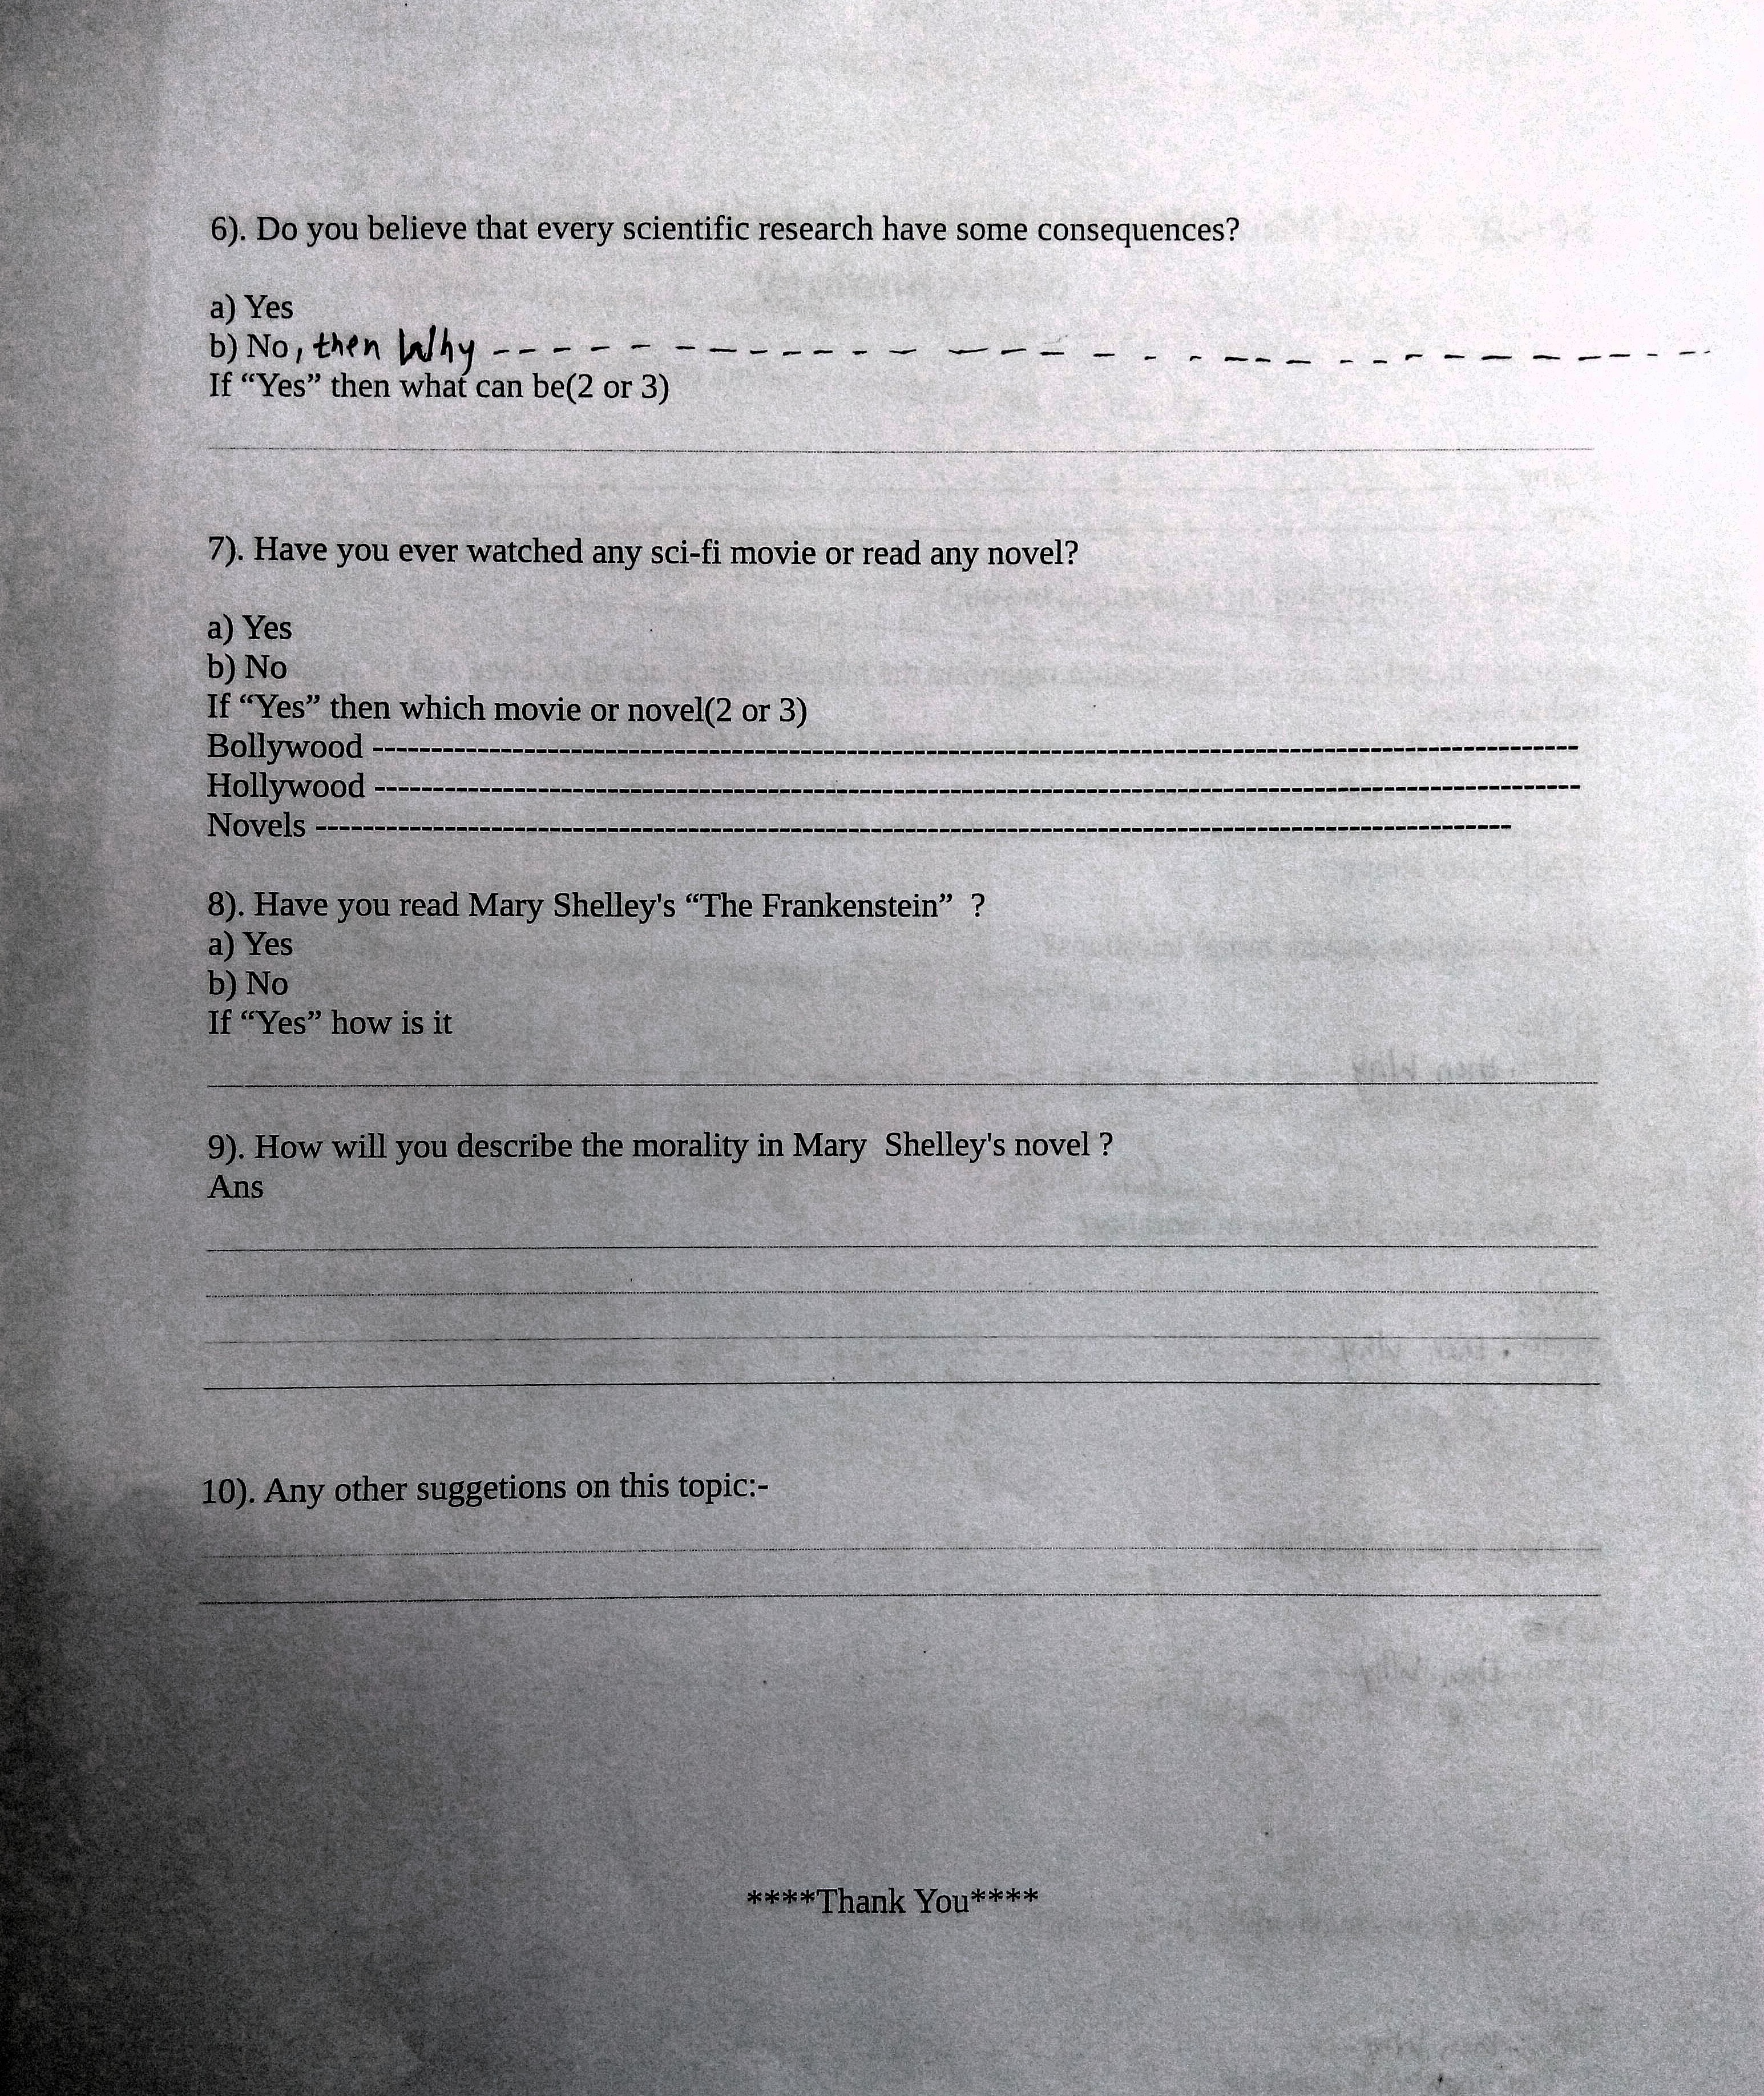
\includegraphics[width=6in,height=9in]{a2.jpg}

\subsection{Appendix-B}
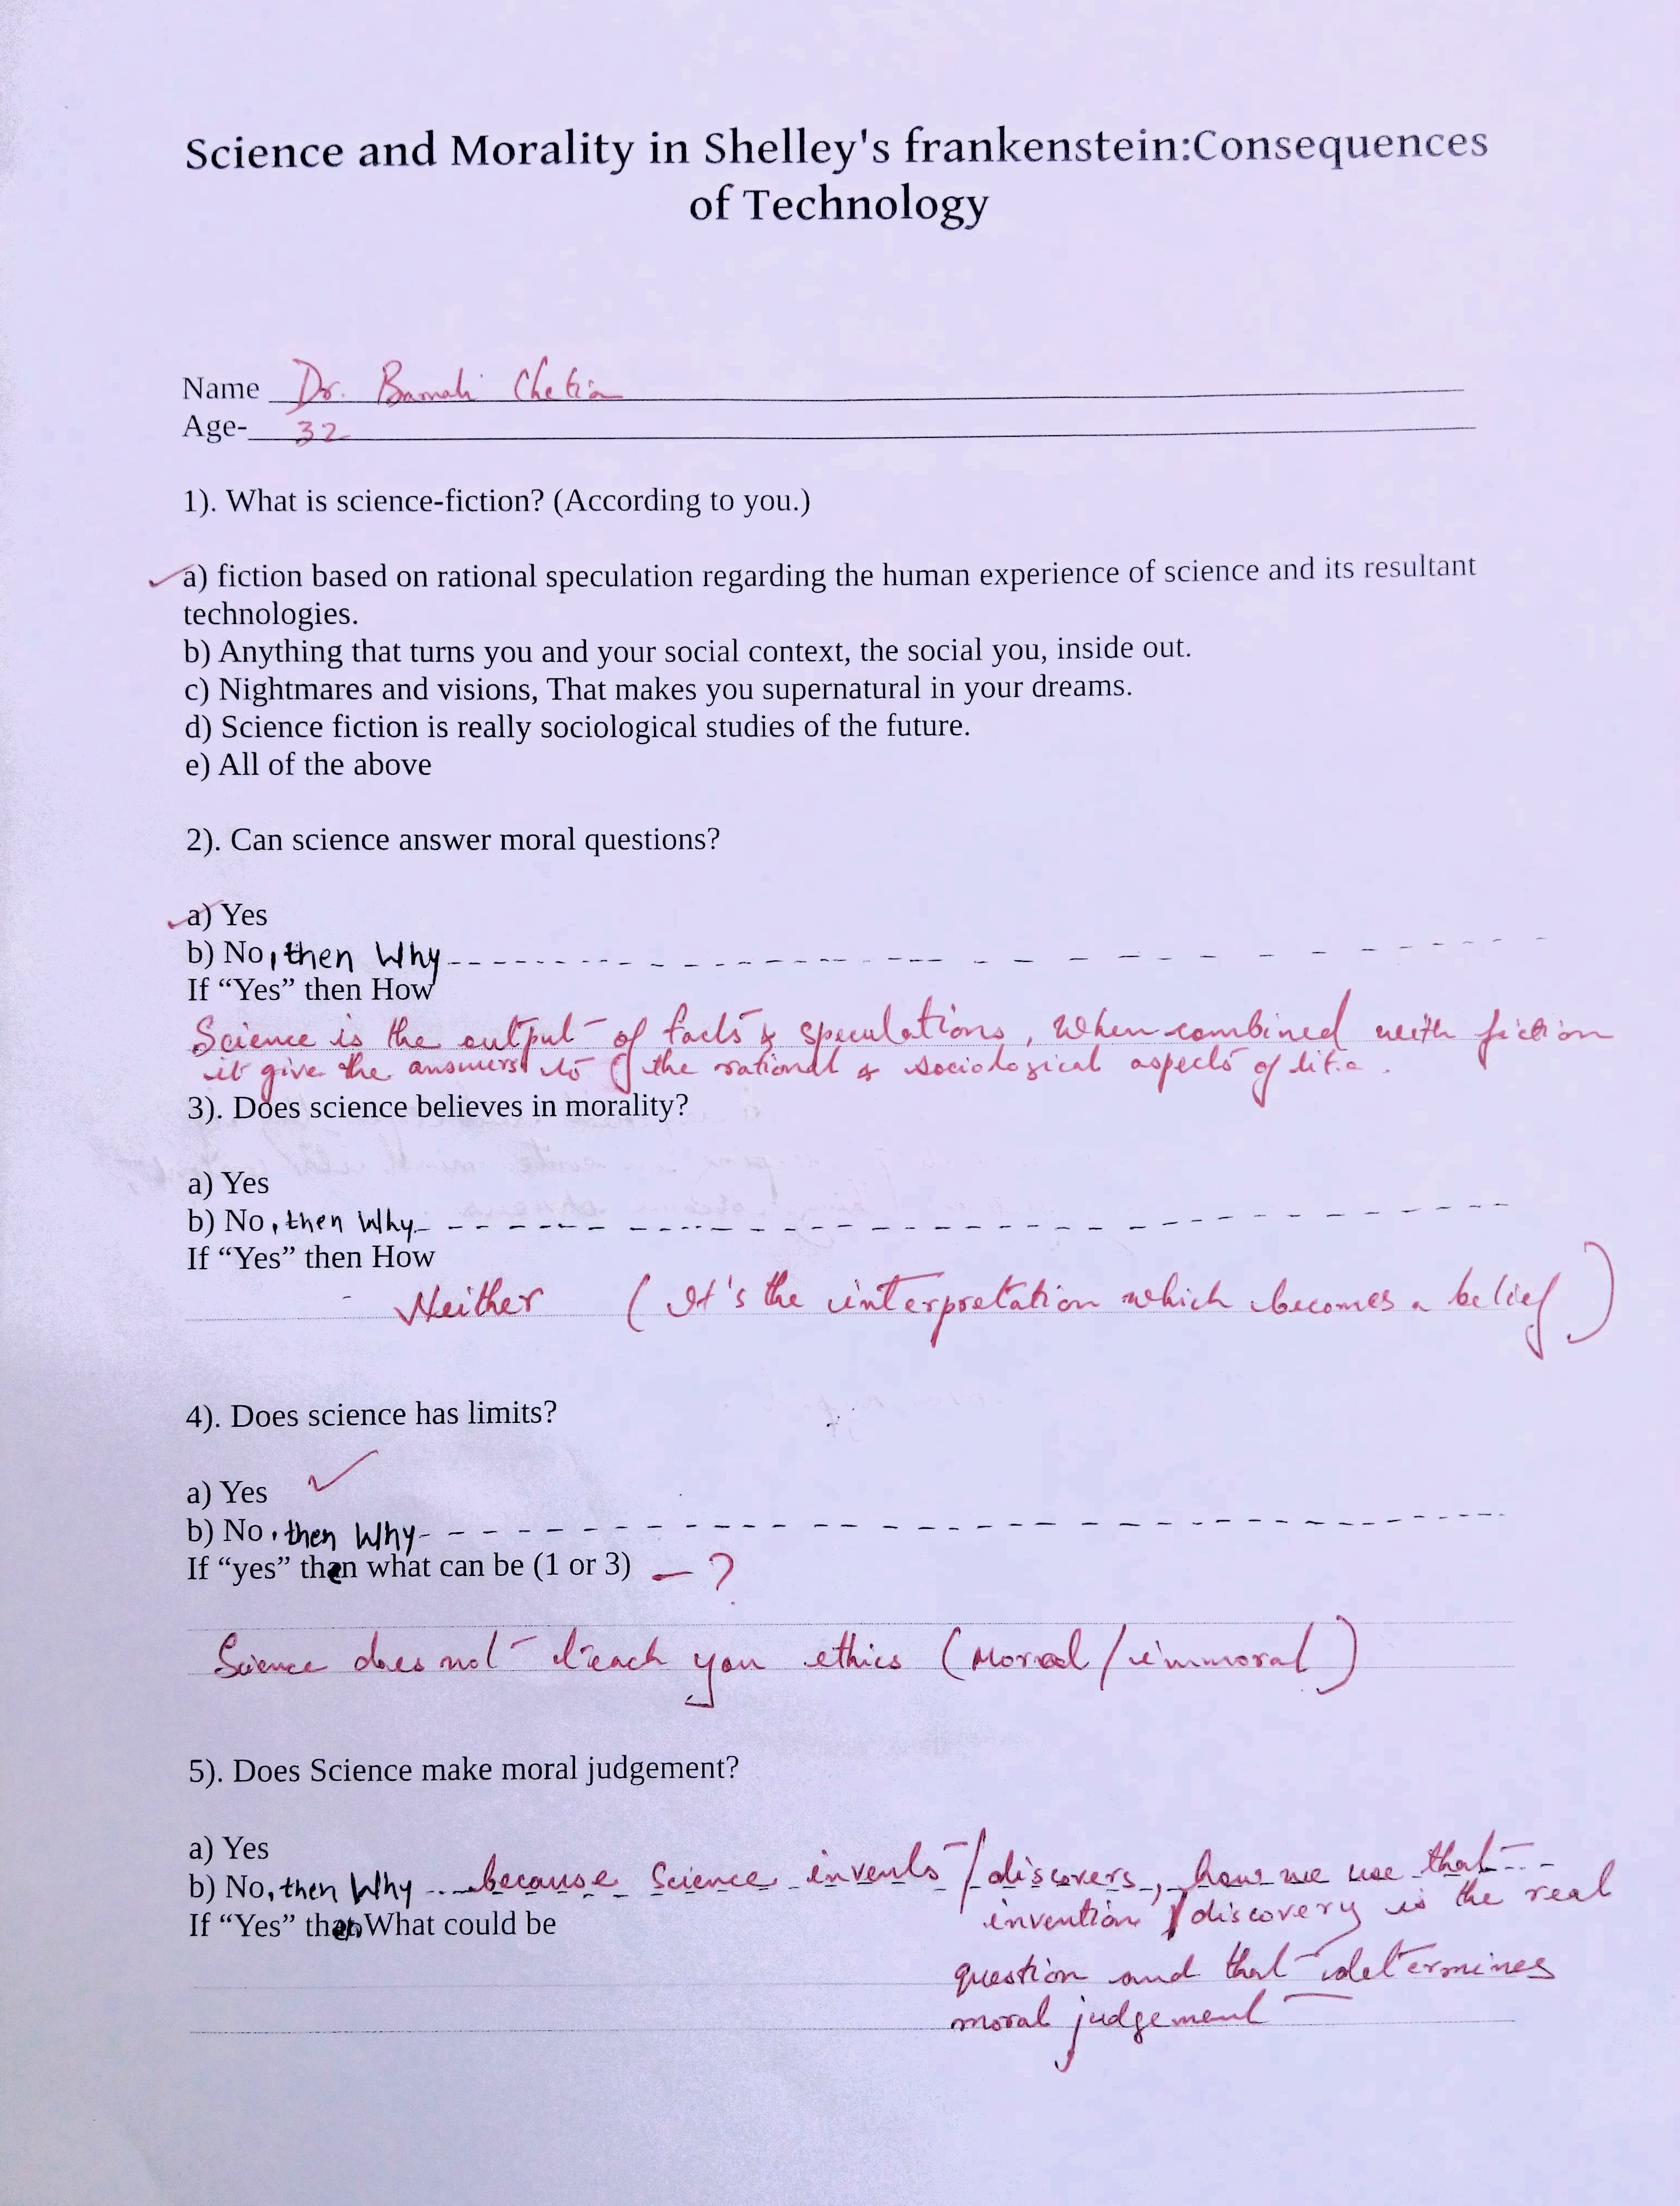
\includegraphics[width=6in,height=9in]{a3.jpg}

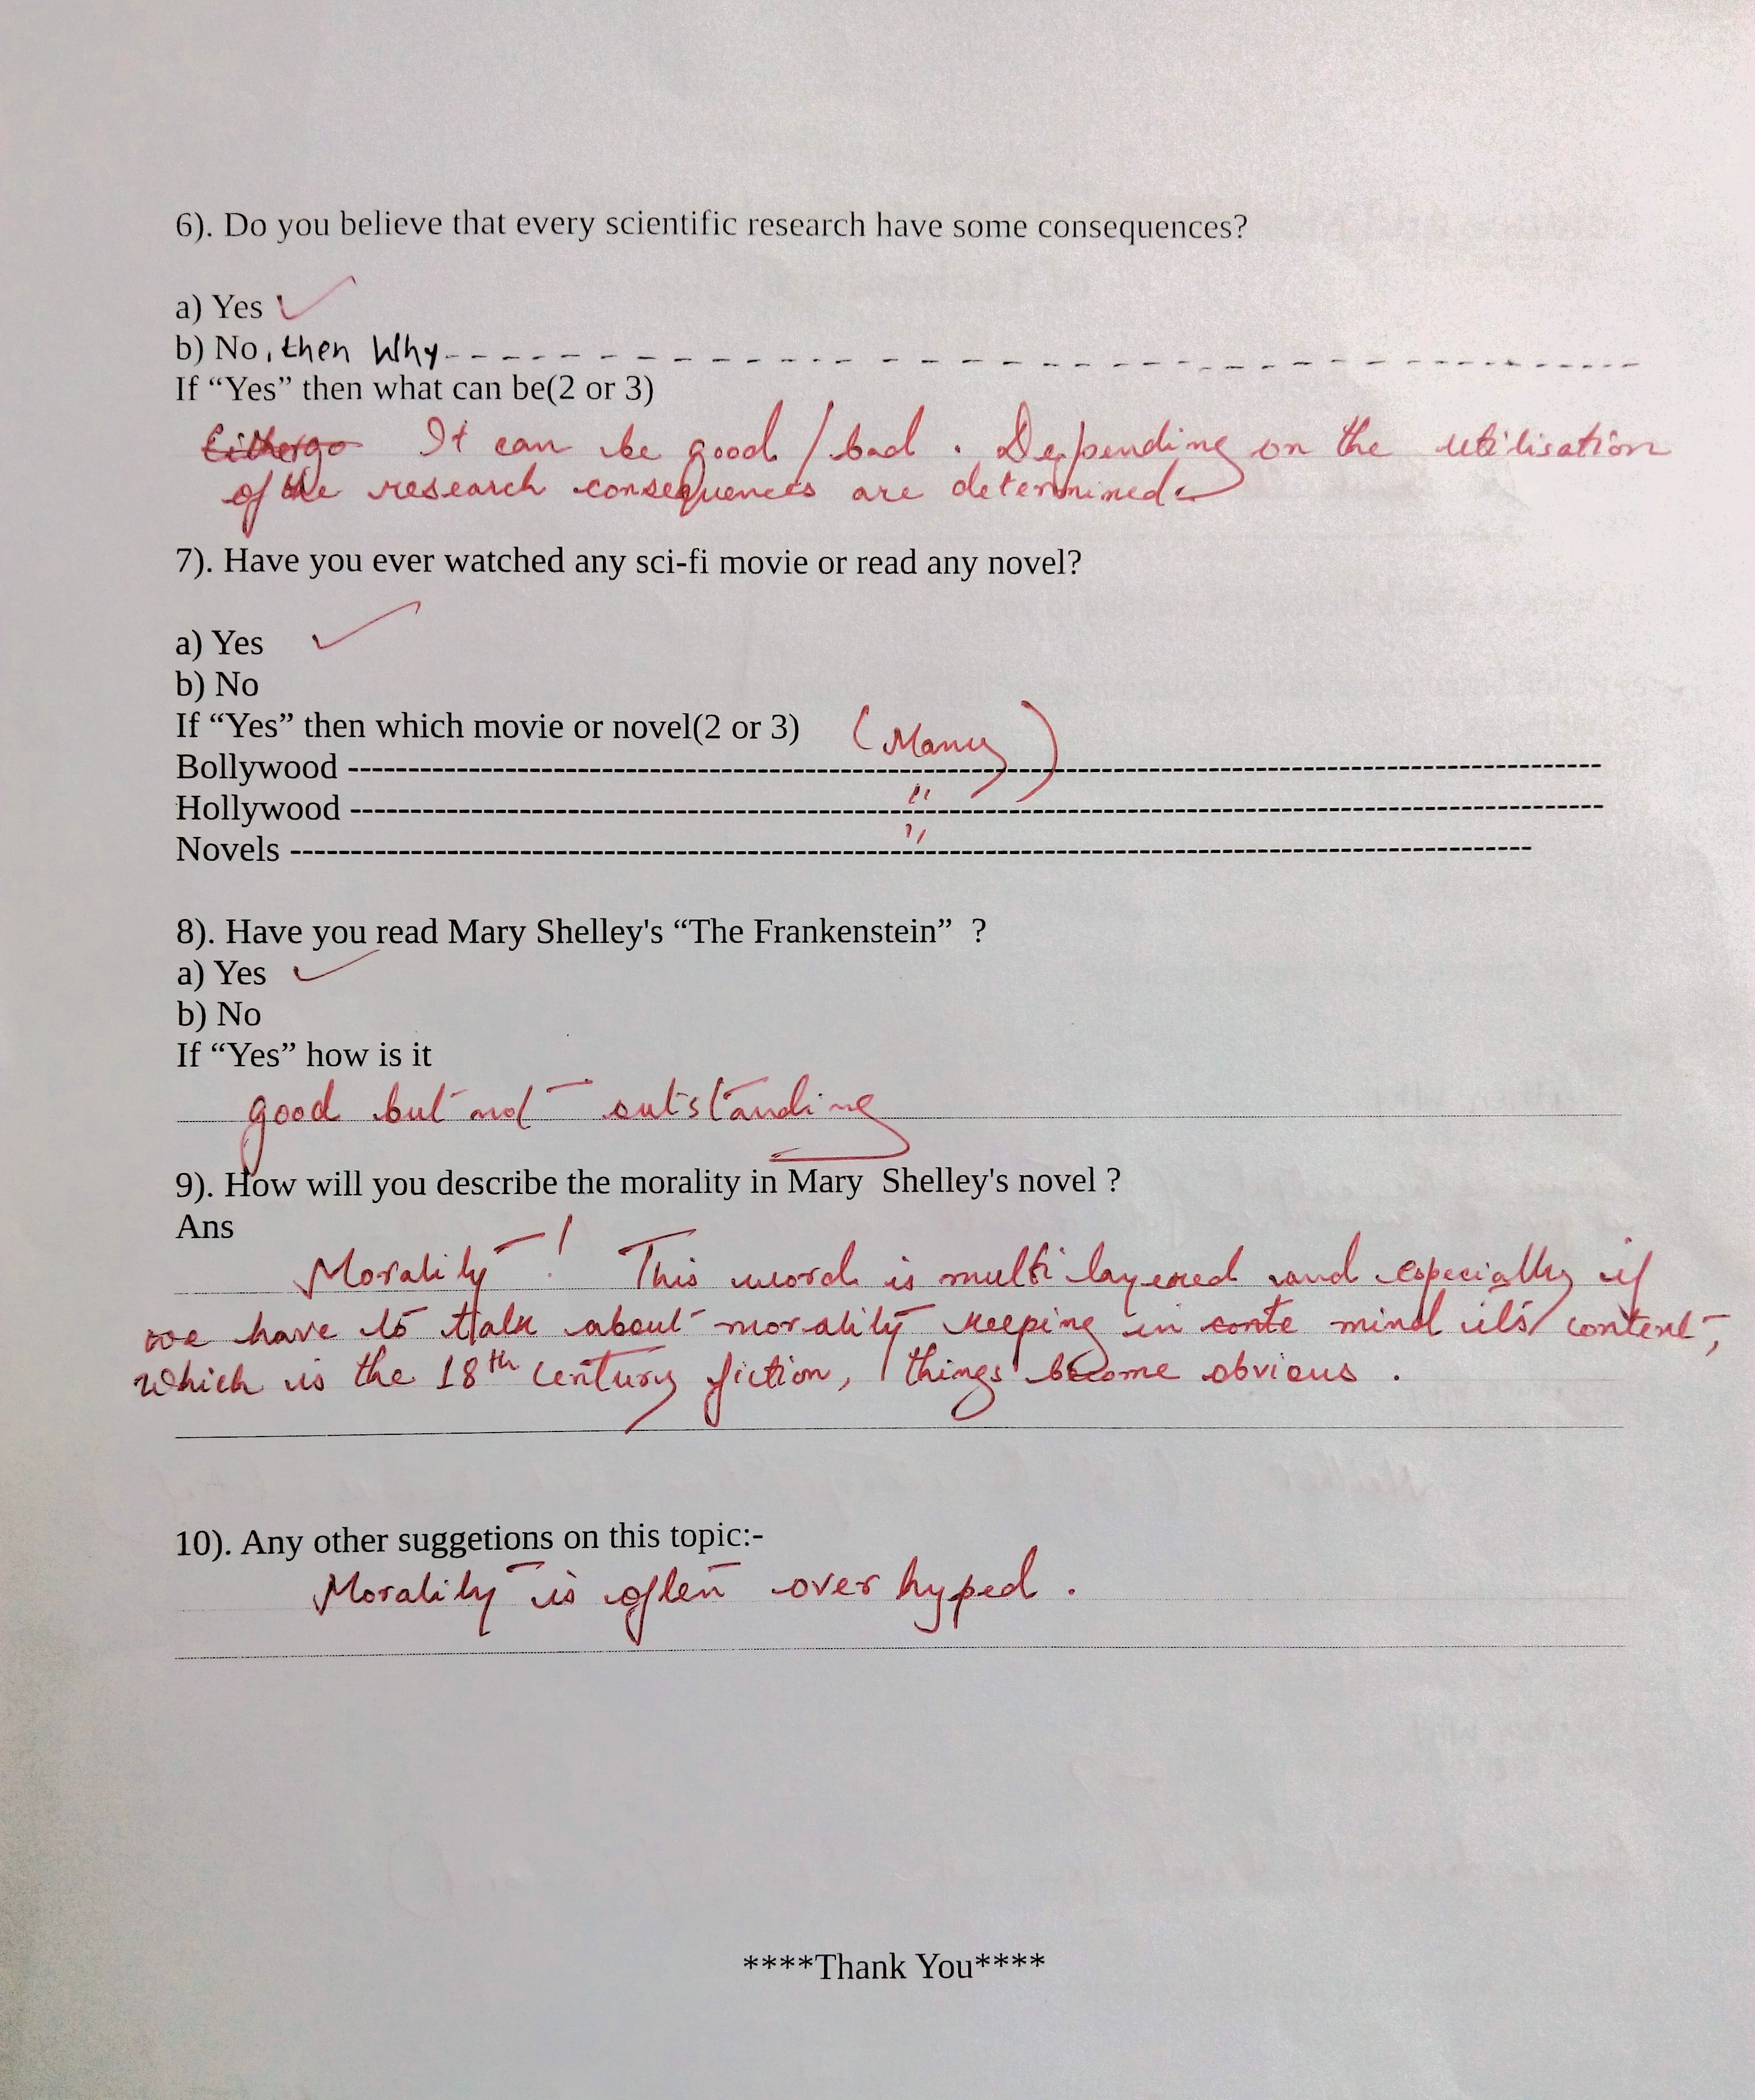
\includegraphics[width=6in,height=9in]{a4.jpg}

\end{document}

